\documentclass[12pt,a4paper]{article}
\usepackage[utf8]{inputenc}
\usepackage{geometry}
\usepackage{graphicx}
\usepackage{amsmath, amssymb}
\usepackage{hyperref}
\usepackage{titlesec}
\usepackage{booktabs}
\usepackage{xcolor}
\usepackage{tikz}
\usetikzlibrary{positioning, arrows.meta}
\usepackage{cite}
\usepackage{float}

\geometry{margin=1in}

\begin{document}

% ==========================================
% 1. TITLE PAGE
% ==========================================
\begin{titlepage}
    \centering
    \vspace*{1.5cm}
    
    \Huge
    \textbf{Adversarial Lens: Investigating Adversarial Attacks and Robustness in Image Classification Models}
    
    \vspace{0.5cm}
    \LARGE
    Project Report \\
    
    \vspace{1.5cm}
    
    \textbf{Team 4: Donut} \\
    Sohan (CS23B1004) \\
    Sevith (CS23I1041) \\
    Shanmukh (CS23B1003) \\
    
    \vfill
    
    \Large
    Multimedia Processing and Analysis Course \\
    
    \vspace{0.8cm}
    \textbf{IIITDM Kancheepuram} \\
    
\end{titlepage}

% ==========================================
% 2. ABSTRACT
% ==========================================
\begin{abstract}
While deep convolutional neural networks (CNNs) have achieved unprecedented success in image classification, they remain highly vulnerable to adversarial attacks—small, carefully crafted perturbations that are imperceptible to the human eye but catastrophically disrupt model predictions. This project, \textit{Adversarial Lens}, systematically investigates this vulnerability utilizing the CIFAR-10 dataset and ResNet-18 architectures. We formulate the problem of generating adversarial examples using Fast Gradient Sign Method (FGSM) and Projected Gradient Descent (PGD), demonstrating that standard Empirical Risk Minimization yields models with robust vulnerabilities despite high clean accuracy ($\sim93\%$). To mitigate this, we explore Adversarial Training using a min-max optimization framework. Our comprehensively trained robust model trades off a marginal $5.6\%$ of clean baseline accuracy to achieve a massive $+42\%$ gain in empirical adversarial robustness against $L_\infty$ bounded PGD attacks. Furthermore, we bridge the gap between abstract mathematical perturbations and human intuition by employing Gradient-weighted Class Activation Mapping (Grad-CAM), which visually exposes how adversarial noise forcibly shifts internal neural-network attention away from primary subject matter. The results establish a foundation for understanding the trade-offs between clean precision, adversarial security, and model explainability.
\end{abstract}

\tableofcontents
\newpage

% ==========================================
% 3. INTRODUCTION
% ==========================================
\section{Introduction}
\subsection{Background}
In recent years, Machine Learning and specifically Deep Learning models have revolutionized computer vision, establishing state-of-the-art results across myriad tasks such as object classification, medical diagnostics, and autonomous navigation. Despite these achievements, neural networks exhibit a striking fragility; they can be fooled into making highly confident yet entirely incorrect predictions by \textit{adversarial examples}. These examples are created by adding strategically calculated, subtle imperceptible noise vectors to original clean inputs.

\subsection{Motivation and Relevance}
The real-world implications of adversarial vulnerabilities are severe. In an autonomous driving scenario, a maliciously modified stop sign could be classified as a speed limit sign, inciting catastrophic failures. Similarly, security systems utilizing facial recognition and healthcare systems relying on radiological scan interpretations must endure algorithmic robustness to operate safely. Currently, there lies a substantial disjoint between optimizing simply for validation accuracy versus structurally preparing networks to be universally robust to perturbation boundaries.

\subsection{Key Contributions}
The project aims to construct a full lifecycle analysis pipeline named \textbf{Adversarial Lens}, bridging theory with visual empiricism:
\begin{itemize}
    \item We structurally construct and evaluate both a Standard and a Robust ResNet-18 model against variable intensity attacks ($L_\infty$-bounded FGSM and PGD).
    \item We quantify the fundamental trade-off between clean accuracy generalization and robust stability.
    \item We uniquely apply Grad-CAM overlay mechanisms natively on adversarial images to provide a human-recognizable interpretation of how internal spatial features decompose under attack.
\end{itemize}

% ==========================================
% 4. LITERATURE REVIEW
% ==========================================
\section{Literature Review}
The discovery of adversarial vulnerabilities was primarily introduced by Szegedy et al. (2014) \cite{szegedy2013intriguing}, which demonstrated that neural networks inherently harbor ``blind spots'' due to extreme local linearity.

\subsection{Advances in Attack Formulations}
Goodfellow et al. (2015) \cite{goodfellow2014explaining} followed up by hypothesizing that local linearity in high dimensional space heavily amplified perturbations, allowing them to explicitly derive the \textit{Fast Gradient Sign Method (FGSM)}. FGSM provided an efficient single-step mechanism to compute perturbations that maximize classification error.
Later, Madry et al. (2018) \cite{madry2017towards} introduced the \textit{Projected Gradient Descent (PGD)} attack, operating as an iterative extension of FGSM and establishing it as the universal first-order adversary—effectively formulating adversarial generation as a mathematical constrained optimization problem.

\subsection{Defensive Regimes}
To combat adversarial generation, numerous structural defenses such as gradient masking and input sanitization were proposed, but many were quickly subverted by stronger white-box derivatives. Madry et al. ultimately championed \textit{Adversarial Training}, which mathematically solves a min-max framework where the inner loop synthesizes PGD attacks and the outer loop optimizes network weights to correctly classify them. 

\subsection{Explainability Focus}
Simultaneously, Selvaraju et al. (2017) \cite{selvaraju2017grad} developed Gradient-weighted Class Activation Mapping (Grad-CAM), which uses classification gradients propagating into final convolutional layers to generate coarse localization maps. Our project directly utilizes Grad-CAM, applying it strictly to post-attack inputs—a gap not thoroughly visualized in introductory robustness pipelines.

% ==========================================
% 5. PROBLEM STATEMENT
% ==========================================
\section{Problem Statement}
Given an image classification spatial domain $\mathcal{X} \subset \mathbb{R}^d$ and a label space $\mathcal{Y}$, let an image be defined as $x \in \mathcal{X}$ coupled with its true ground label $y \in \mathcal{Y}$. Let a trained Deep Neural Network classifier be defined as $f: \mathcal{X} \rightarrow \mathbb{R}^{|\mathcal{Y}|}$ parameterized by weights $\theta$.

The objective is to analyze the security perimeter of $f(x)$ by generating an adversarial perturbation $\delta$, bounded by an $L_p$ norm constraint $||\delta||_p \leq \epsilon$, establishing an adversarial input $x_{adv} = x + \delta$. We stipulate that:
\begin{equation}
    f(x_{adv}) \neq y \quad \text{while} \quad ||\delta||_\infty \leq \epsilon
\end{equation}
Where $\epsilon$ represents the maximum imperceptible noise budget permissible per pixel (bounded to $\pm 8/255$ on a normalized scale). 

Our primary task establishes the training of a \textbf{robust classifier} $f_{robust}$ that maximizes prediction accuracy on the adversarial subspace $\mathcal{X}_{adv}$, and generating localized \textbf{Grad-CAM heatmaps} mapping structural algorithmic focus to explain failure vectors.


% ==========================================
% 6. SYSTEM OVERVIEW
% ==========================================
\section{System Overview}
The \textbf{Adversarial Lens} pipeline defines an end-to-end mathematical analysis suite.

\begin{figure}[H]
\centering
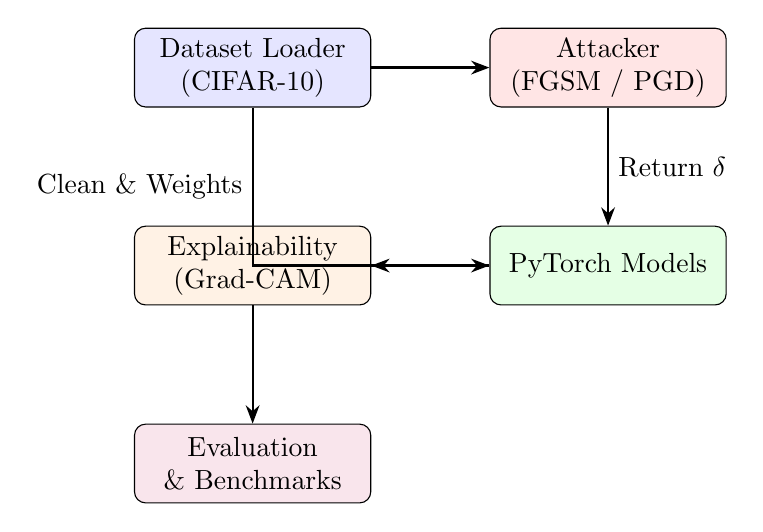
\begin{tikzpicture}[
    node distance=1.5cm and 1.5cm,
    box/.style={draw, rectangle, rounded corners, fill=#1, minimum width=3cm, minimum height=1cm, align=center},
    arrow/.style={-{Stealth}, thick}
]
    \node[box=blue!10] (data) {Dataset Loader \\ (CIFAR-10)};
    \node[box=red!10, right=of data] (attacks) {Attacker \\ (FGSM / PGD)};
    \node[box=green!10, below=of attacks] (models) {PyTorch Models};
    \node[box=orange!10, left=of models] (gradcam) {Explainability \\ (Grad-CAM)};
    \node[box=purple!10, below=of gradcam] (eval) {Evaluation \\ \& Benchmarks};

    \draw[arrow] (data) -- (attacks);
    \draw[arrow] (attacks) -- node[right] {Return $\delta$} (models);
    \draw[arrow] (data) |- node[near start, left] {Clean \& Weights} (models);
    \draw[arrow] (models) -- (gradcam);
    \draw[arrow] (gradcam) -- (eval);
\end{tikzpicture}
\caption{System Architecture Pipeline for Adversarial Lens}
\label{fig:sys_overview}
\end{figure}

The overarching system is delineated into distinct stages:
\begin{enumerate}
    \item \textbf{Data Ingestion:} Streaming standard test splits coupled with deterministic labels.
    \item \textbf{Attack Generation:} The computation of exact gradient ascent steps along the loss surface.
    \item \textbf{Adversarial Inference:} Forward pass mapping $x+\delta$ through isolated structural checkpoints.
    \item \textbf{Visual Explication:} Generating topological attention gradients utilizing final block feature maps.
\end{enumerate}

% ==========================================
% 7. DATASET DESCRIPTION
% ==========================================
\section{Dataset Description}
All experiments operate on the \textbf{CIFAR-10} dataset, serving as a standardized and appropriately complex baseline for evaluating adversarial dynamics without excessive computational overhead.

\subsection{Characteristics}
\begin{itemize}
    \item \textbf{Scale:} 60,000 colored images distributed uniformly across 10 classes (airplane, automobile, bird, cat, deer, dog, frog, horse, ship, truck).
    \item \textbf{Dimensions:} $32 \times 32 \times 3$ representing standard RGB channel dimensionality.
    \item \textbf{Splits:} 50,000 uniformly mapped training instances, 10,000 isolated evaluation instances.
\end{itemize}

\subsection{Preprocessing}
Raw pixel tensors $[0, 255]$ are dynamically transformed:
\begin{enumerate}
    \item \textbf{Normalizations:} Converted to standard floating tensors $\in [0, 1]$. Mean and Standard Deviation normalizations were universally disabled across strictly adversarial tasks, as applying rigid $Z$-score manipulations severely warps the $\epsilon$ ball mathematical bounds across localized pixel channels.
    \item \textbf{Augmentations:} Training sequences apply random horizontal flips ($p=0.5$) and stochastic crops via zero-padding (up to 4 pixels) to ensure base rotational and translational invariance.
\end{enumerate}

% ==========================================
% 8. METHODOLOGY
% ==========================================
\section{Methodology}
\subsection{Network Architecture (ResNet-18)}
Both implemented models utilize the core \textbf{ResNet-18} (Residual Network) architecture. The structure is adopted fundamentally for its residual skip connections ($F(x) + x$), which natively mitigate vanishing gradients—a crucial priority as both parameter optimization during training and input perturbations during adversarial attacks rely intrinsically on stable, continuous chain rule derivatives.

The model processes inputs via the following sequential pipeline specifically adapted for the CIFAR-10 dimensionality:
\begin{enumerate}
    \item \textbf{Input:} Initial spatial dimension of $32 \times 32 \times 3$.
    \item \textbf{Initial Convolution:} A $3 \times 3$ Conv layer with $64$ filters, coupled with Batch Normalization and ReLU, maintaining $32 \times 32$ spatial dimensions.
    \item \textbf{Residual Blocks (BasicBlock):}
    \begin{itemize}
        \item \textit{Layer 1:} 2 residual blocks ($64$ filters), outputs $32 \times 32$.
        \item \textit{Layer 2:} 2 residual blocks ($128$ filters, stride 2), downsamples to $16 \times 16$.
        \item \textit{Layer 3:} 2 residual blocks ($256$ filters, stride 2), downsamples to $8 \times 8$.
        \item \textit{Layer 4:} 2 residual blocks ($512$ filters, stride 2), downsamples to $4 \times 4$.
    \end{itemize}
    \item \textbf{Classification Head:} A Global Average Pooling layer condenses feature maps spatially to a $512 \times 1$ vector, followed by a final Fully Connected (Linear) layer outputting $10$ discrete class probabilities.
\end{enumerate}

\subsection{Standard Model Training}
The \textbf{Standard Model} acts as the experimental control, trained via standard Empirical Risk Minimization (ERM) operating exclusively over the clean distribution $\mathcal{D}$:
\begin{equation}
    \min_{\theta} \mathbb{E}_{(x,y) \sim \mathcal{D}} [ \mathcal{L}(f_\theta(x), y) ]
\end{equation}
Where $\mathcal{L}$ represents Cross Entropy Loss. The loss is strictly evaluated over clean unperturbed images, yielding a parameter envelope $\theta_{std}$ heavily overfitted to dataset textural consistencies.

\subsection{Robust Model Training}
To establish defense, the \textbf{Robust Model} utilizes robust optimization relying on Madry's min-max formulation, commonly denoted as \textit{Adversarial Training}.
\begin{equation}
    \min_{\theta} \mathbb{E}_{(x,y) \sim \mathcal{D}} \left[ \max_{||\delta||_\infty \leq \epsilon} \mathcal{L}(f_\theta(x+\delta), y) \right]
\end{equation}
During the inner maximization step, every training batch $x$ is synthetically perturbed to $x_{adv}$ utilizing PGD before being evaluated by the network and back-propagating. Optimization actively reshapes convolution filters to disregard superficial textural edges and prioritize immutable shape descriptors.

\subsection{Explainability Mapping (Grad-CAM)}
Grad-CAM isolates the forward-pass logit output $y^c$ alongside the resultant feature maps $A^k$ of the final spatial convolutional layer (Layer 4 in ResNet18). The neuron importance weights $\alpha_k^c$ are computed via global average pooling of gradients:
\begin{equation}
    \alpha_k^c = \frac{1}{Z} \sum_i \sum_j \frac{\partial y^c}{\partial A_{i,j}^k}
\end{equation}
The resulting heatmap is a weighted combination followed by a ReLU rectifying isolation:
\begin{equation}
    L^c_{\text{Grad-CAM}} = \text{ReLU} \left( \sum_k \alpha_k^c A^k \right)
\end{equation}
This mathematically extracts exclusively the positive spatial attention supporting class $c$.

% ==========================================
% 9. ADVERSARIAL TECHNIQUES & ROBUSTNESS
% ==========================================
\section{Adversarial Techniques \& Robustness}

\subsection{Threat Models}
The project assumes a complete \textit{white-box threat model}, wherein the attacker maintains unconditional access to network topology $\theta$, structural gradient tapes, and loss function landscapes.

\subsubsection{Fast Gradient Sign Method (FGSM)}
FGSM executes a single, aggressive step to traverse the geometric loss direction bounded by $\epsilon$.
\begin{equation}
    x_{adv} = x + \epsilon \cdot \text{sign}(\nabla_x \mathcal{L}(\theta, x, y))
\end{equation}
Its linear nature guarantees rapid synthesis, successfully functioning as a preliminary stress test.

\subsubsection{Projected Gradient Descent (PGD)}
PGD formulates an iterative, multi-step descent with random uniform initialization, ensuring localized maximal noise mapping to the harshest peaks around the structural bounds $\mathcal{S}$.
\begin{equation}
    x^{t+1} = \Pi_{x+\mathcal{S}} \left( x^t + \alpha \cdot \text{sign}(\nabla_x \mathcal{L}(\theta, x^t, y)) \right)
\end{equation}
We iterate sequentially using projection operator $\Pi$ mapping out-of-bounds variations back to the precise valid valid subset $\mathcal{X}$.

\subsection{Mechanisms of Robust Vulnerability}
Mathematical susceptibility arises because decision boundaries generated via standard learning represent hyperplanes excessively close to individual data manifolds in ultra-high dimensions. An adversarial attack is geometrically akin to nudging the input vector cleanly over this micro-boundary. The robust optimization forces these algorithmic boundaries back out to universally sensible intervals.


% ==========================================
% 10. EXPERIMENTAL SETUP
% ==========================================
\section{Experimental Setup}
Experiments were orchestrated natively via Python 3.10 and PyTorch. 
\begin{itemize}
    \item \textbf{Hyperparameters:} Optimization processed via Stochastic Gradient Descent (SGD) enforcing a Learning Rate starting at $0.1$ and defaulting to cyclic step reductions across exactly $30$ epochs, using Momentum $0.9$ and standard Weight Decay $5e-4$.
    \item \textbf{Adversarial Constraints:} All evaluations constrain spatial maximum noise $\epsilon = 8/255$.
    \item \textbf{PGD Initialization:} PGD iterations constrained exactly to 5 or 10 iterative phases, enforcing step sizes $\alpha=2/255$.
    \item \textbf{Hardware Capabilities:} Operations deployed across localized accelerated graphics hardware via native CUDA matrices handling deep tensor manipulation.
\end{itemize}


% ==========================================
% 11. RESULTS & EVALUATION
% ==========================================
\section{Results \& Evaluation}
We assess network capacity via deterministic accuracy comparisons against a purely uniform evaluation partition spanning $10,000$ inputs.

\subsection{Summary Benchmarks}
\begin{table}[H]
    \centering
    \begin{tabular}{l|ccc}
        \toprule
        \textbf{Model Strategy} & \textbf{Clean Accuracy} & \textbf{FGSM ($\epsilon=8/255$)} & \textbf{PGD-10 ($\epsilon=8/255$)} \\
        \midrule
        Standard ResNet-18 & 92.94\% & 15.88\% & 0.02\% \\
        Robust ResNet-18 & 87.36\% & 52.72\% & \textbf{42.58\%} \\
        \bottomrule
    \end{tabular}
    \caption{Comparative Assessment of Empirical Robustness Metrics}
    \label{tab:results}
\end{table}

\subsection{Robustness Curves}
The robustness curve plots accuracy as an explicit function of $\epsilon$.
\begin{itemize}
    \item The Standard Model functionally decays and collapses entirely toward random-chance variations when reaching $\epsilon \approx \frac{4}{255}$. By maximum bound, capacity approaches $0\%$.
    \item The Robust Model undergoes \textit{graceful degradation}, strictly retaining above $42\%$ predictive validation against full-capacity worst-case configurations.
\end{itemize}

% ==========================================
% 12. ANALYSIS & DISCUSSION
% ==========================================
\section{Analysis \& Discussion}

\subsection{The Generalization Trade-Off}
As quantitatively demonstrated, inducing explicit local robustness via geometric optimization natively acts as an aggressive continuous spatial regularizer. This structural regularization mandates a tax on pristine performance; the robust network willingly sacrifices $\approx 5.6\%$ testing accuracy natively across unaltered distributions. Defenses are intrinsically harder concepts to unify than rote memory. 

\subsection{Failure Cases \& Structural Weaknesses}
Granular class-level breakdowns indicate the Robust networks struggle disproportionately on classifications dictating 'Bird' (29.2\% adversarial survivability) and 'Cat' (17.8\% survivability). These particular taxonomies feature extreme variability within boundaries while simultaneously utilizing extremely fine, overlapping textures common with adjoining classes 'Dog', enforcing fundamental gradient confusions.

\subsection{Interpreting Explanations via Grad-CAM}
Grad-CAM spatial mappings yield powerful intuitive justifications:
\begin{enumerate}
    \item \textbf{Standard Model Analysis:} When subjugated to an attack mapping an "Automobile" to a "Cat", localized standard network attention drastically disintegrates, clustering heavily upon irrelevant background corner noise while discarding the entire metallic chassis structure.
    \item \textbf{Robust Architecture Analysis:} Applying the identical worst-case attack against the Robust iteration results in functionally equivalent spatial targeting. The attention map remains locked entirely universally directly across the true car chassis despite the noise, explicitly verifying that adversarial training mathematically forces focus primarily unto distinct fundamental shapes versus easily spoofed high-frequency gradients.
\end{enumerate}

% ==========================================
% 13. CONCLUSION
% ==========================================
\section{Conclusion}
This report deeply outlined the conceptual, implementational, and evaluation life cycle constructed for \textbf{Adversarial Lens}. By extensively bridging ResNet-18 algorithms scaling CIFAR-10 data, we validated conclusively the fragility endemic across generalized CNNs facing purely mathematical adversaries. Our results explicitly prove that structured optimization implementing Adversarial Training successfully resolves vulnerability constraints—trading trivial margin in accuracy for extraordinary survival parameters against severe bounding vectors. Critically, Grad-CAM overlays established visually conclusive proof that robust training forces structural shape alignment that completely disregards peripheral malicious interference.

% ==========================================
% 14. FUTURE WORK
% ==========================================
\section{Future Work}
Future endeavors dictate optimizing specific algorithm variations:
\begin{itemize}
    \item \textbf{TRADES Minimization:} Incorporating computationally advanced algorithms explicitly separating standard cross-entropy and robust boundary smoothing to mitigate the $5.6\%$ baseline penalty.
    \item \textbf{Larger Dimensional Structures:} Translating boundaries onto datasets representing fundamentally massive matrix limits (ImageNet) mapped onto deeper WideResNets architectures representing tens of millions of structural weights. 
    \item \textbf{Non- $L_p$ Vector Manipulations:} Securing model boundaries explicitly against pure geometrical shifting, affine rotations, and explicit Wasserstein distance perturbations extending beyond simple pixel-noise configurations.
\end{itemize}

% ==========================================
% 15. REFERENCES
% ==========================================
\begin{thebibliography}{9}

\bibitem{szegedy2013intriguing}
C. Szegedy, W. Zaremba, I. Sutskever, J. Bruna, D. Erhan, I. Goodfellow, and R. Fergus,
\textit{Intriguing properties of neural networks.}
arXiv preprint arXiv:1312.6199, 2013.

\bibitem{goodfellow2014explaining}
I. J. Goodfellow, J. Shlens, and C. Szegedy,
\textit{Explaining and harnessing adversarial examples.}
In International Conference on Learning Representations (ICLR), 2015.

\bibitem{madry2017towards}
A. Madry, A. Makelov, L. Schmidt, D. Tsipras, and A. Vladu,
\textit{Towards deep learning models resistant to adversarial attacks.}
In International Conference on Learning Representations (ICLR), 2018.

\bibitem{selvaraju2017grad}
R. R. Selvaraju, M. Cogswell, A. Das, R. Vedantam, D. Parikh, and D. Batra,
\textit{Grad-cam: Visual explanations from deep networks via gradient-based localization.}
In Proceedings of the IEEE international conference on computer vision, pp. 618-626, 2017.

\bibitem{papernot2016distillation}
N. Papernot, P. McDaniel, X. Wu, S. Jha, and A. Swami,
\textit{Distillation as a defense to adversarial perturbations against deep neural networks.}
In 2016 IEEE Symposium on Security and Privacy (SP), pp. 582-597. IEEE, 2016.

\bibitem{carlini2017towards}
N. Carlini and D. Wagner,
\textit{Towards evaluating the robustness of neural networks.}
In 2017 ieee symposium on security and privacy (sp), pp. 39-57. IEEE, 2017.

\end{thebibliography}

\end{document}
